% Options for packages loaded elsewhere
% Options for packages loaded elsewhere
\PassOptionsToPackage{unicode}{hyperref}
\PassOptionsToPackage{hyphens}{url}
\PassOptionsToPackage{dvipsnames,svgnames,x11names}{xcolor}
%
\documentclass[
  letterpaper,
  DIV=11,
  numbers=noendperiod]{scrartcl}
\usepackage{xcolor}
\usepackage{amsmath,amssymb}
\setcounter{secnumdepth}{5}
\usepackage{iftex}
\ifPDFTeX
  \usepackage[T1]{fontenc}
  \usepackage[utf8]{inputenc}
  \usepackage{textcomp} % provide euro and other symbols
\else % if luatex or xetex
  \usepackage{unicode-math} % this also loads fontspec
  \defaultfontfeatures{Scale=MatchLowercase}
  \defaultfontfeatures[\rmfamily]{Ligatures=TeX,Scale=1}
\fi
\usepackage{lmodern}
\ifPDFTeX\else
  % xetex/luatex font selection
\fi
% Use upquote if available, for straight quotes in verbatim environments
\IfFileExists{upquote.sty}{\usepackage{upquote}}{}
\IfFileExists{microtype.sty}{% use microtype if available
  \usepackage[]{microtype}
  \UseMicrotypeSet[protrusion]{basicmath} % disable protrusion for tt fonts
}{}
\makeatletter
\@ifundefined{KOMAClassName}{% if non-KOMA class
  \IfFileExists{parskip.sty}{%
    \usepackage{parskip}
  }{% else
    \setlength{\parindent}{0pt}
    \setlength{\parskip}{6pt plus 2pt minus 1pt}}
}{% if KOMA class
  \KOMAoptions{parskip=half}}
\makeatother
% Make \paragraph and \subparagraph free-standing
\makeatletter
\ifx\paragraph\undefined\else
  \let\oldparagraph\paragraph
  \renewcommand{\paragraph}{
    \@ifstar
      \xxxParagraphStar
      \xxxParagraphNoStar
  }
  \newcommand{\xxxParagraphStar}[1]{\oldparagraph*{#1}\mbox{}}
  \newcommand{\xxxParagraphNoStar}[1]{\oldparagraph{#1}\mbox{}}
\fi
\ifx\subparagraph\undefined\else
  \let\oldsubparagraph\subparagraph
  \renewcommand{\subparagraph}{
    \@ifstar
      \xxxSubParagraphStar
      \xxxSubParagraphNoStar
  }
  \newcommand{\xxxSubParagraphStar}[1]{\oldsubparagraph*{#1}\mbox{}}
  \newcommand{\xxxSubParagraphNoStar}[1]{\oldsubparagraph{#1}\mbox{}}
\fi
\makeatother


\usepackage{longtable,booktabs,array}
\newcounter{none} % for unnumbered tables
\usepackage{calc} % for calculating minipage widths
% Correct order of tables after \paragraph or \subparagraph
\usepackage{etoolbox}
\makeatletter
\patchcmd\longtable{\par}{\if@noskipsec\mbox{}\fi\par}{}{}
\makeatother
% Allow footnotes in longtable head/foot
\IfFileExists{footnotehyper.sty}{\usepackage{footnotehyper}}{\usepackage{footnote}}
\makesavenoteenv{longtable}
\usepackage{graphicx}
\makeatletter
\newsavebox\pandoc@box
\newcommand*\pandocbounded[1]{% scales image to fit in text height/width
  \sbox\pandoc@box{#1}%
  \Gscale@div\@tempa{\textheight}{\dimexpr\ht\pandoc@box+\dp\pandoc@box\relax}%
  \Gscale@div\@tempb{\linewidth}{\wd\pandoc@box}%
  \ifdim\@tempb\p@<\@tempa\p@\let\@tempa\@tempb\fi% select the smaller of both
  \ifdim\@tempa\p@<\p@\scalebox{\@tempa}{\usebox\pandoc@box}%
  \else\usebox{\pandoc@box}%
  \fi%
}
% Set default figure placement to htbp
\def\fps@figure{htbp}
\makeatother





\setlength{\emergencystretch}{3em} % prevent overfull lines

\providecommand{\tightlist}{%
  \setlength{\itemsep}{0pt}\setlength{\parskip}{0pt}}



 


\KOMAoption{captions}{tableheading}
\makeatletter
\@ifpackageloaded{caption}{}{\usepackage{caption}}
\AtBeginDocument{%
\ifdefined\contentsname
  \renewcommand*\contentsname{Table of contents}
\else
  \newcommand\contentsname{Table of contents}
\fi
\ifdefined\listfigurename
  \renewcommand*\listfigurename{List of Figures}
\else
  \newcommand\listfigurename{List of Figures}
\fi
\ifdefined\listtablename
  \renewcommand*\listtablename{List of Tables}
\else
  \newcommand\listtablename{List of Tables}
\fi
\ifdefined\figurename
  \renewcommand*\figurename{Figure}
\else
  \newcommand\figurename{Figure}
\fi
\ifdefined\tablename
  \renewcommand*\tablename{Table}
\else
  \newcommand\tablename{Table}
\fi
}
\@ifpackageloaded{float}{}{\usepackage{float}}
\floatstyle{ruled}
\@ifundefined{c@chapter}{\newfloat{codelisting}{h}{lop}}{\newfloat{codelisting}{h}{lop}[chapter]}
\floatname{codelisting}{Listing}
\newcommand*\listoflistings{\listof{codelisting}{List of Listings}}
\makeatother
\makeatletter
\makeatother
\makeatletter
\@ifpackageloaded{caption}{}{\usepackage{caption}}
\@ifpackageloaded{subcaption}{}{\usepackage{subcaption}}
\makeatother
\usepackage{bookmark}
\IfFileExists{xurl.sty}{\usepackage{xurl}}{} % add URL line breaks if available
\urlstyle{same}
\hypersetup{
  pdftitle={About Us},
  colorlinks=true,
  linkcolor={blue},
  filecolor={Maroon},
  citecolor={Blue},
  urlcolor={Blue},
  pdfcreator={LaTeX via pandoc}}


\title{About Us}
\author{}
\date{}
\begin{document}
\maketitle


\protect\phantomsection\label{hero-heading}
\section{\texorpdfstring{\href{https://jonathanwil.com}{Jonathan
Wilson}}{Jonathan Wilson}}\label{jonathan-wilson}

\begin{figure}[H]

{\centering 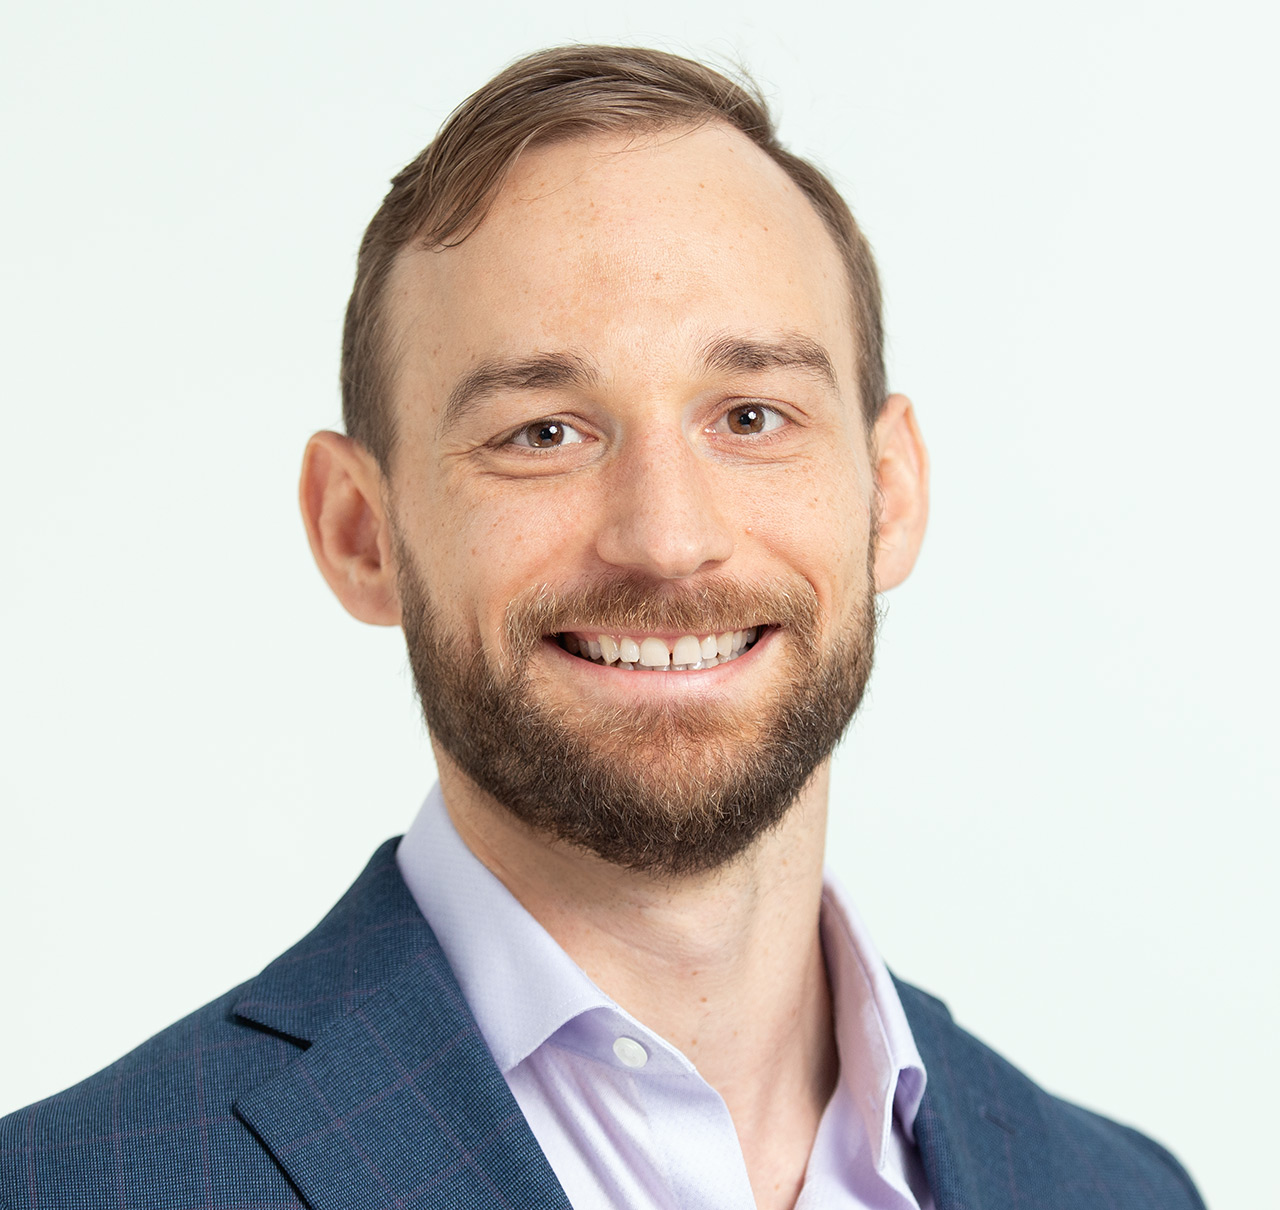
\includegraphics[width=0.28\linewidth,height=\textheight,keepaspectratio,alt={Jonathan Wilson}]{./images/about/jon.png}

}

\caption{Jonathan Wilson}

\end{figure}%

I'm an engineer at heart. I grew up working in construction, earned a
degree in Applied Statistics and Computer Science from BYU, and have
spent more than a decade building software across diverse
domains---ranging from DoD satellites, image processing, optimization,
and large-scale cybersecurity analytics to network engineering,
monitoring, and data platforms. Today, my focus is on designing data
architectures and pipelines for modeling, simulation, and analysis of
large-scale systems. I am currently pursuing a master's in Data
Analytics Engineering at George Mason University.

\section{\texorpdfstring{\href{https://your-link-here.com}{Karan
Lastname}}{Karan Lastname}}\label{karan-lastname}

\begin{figure}[H]

{\centering 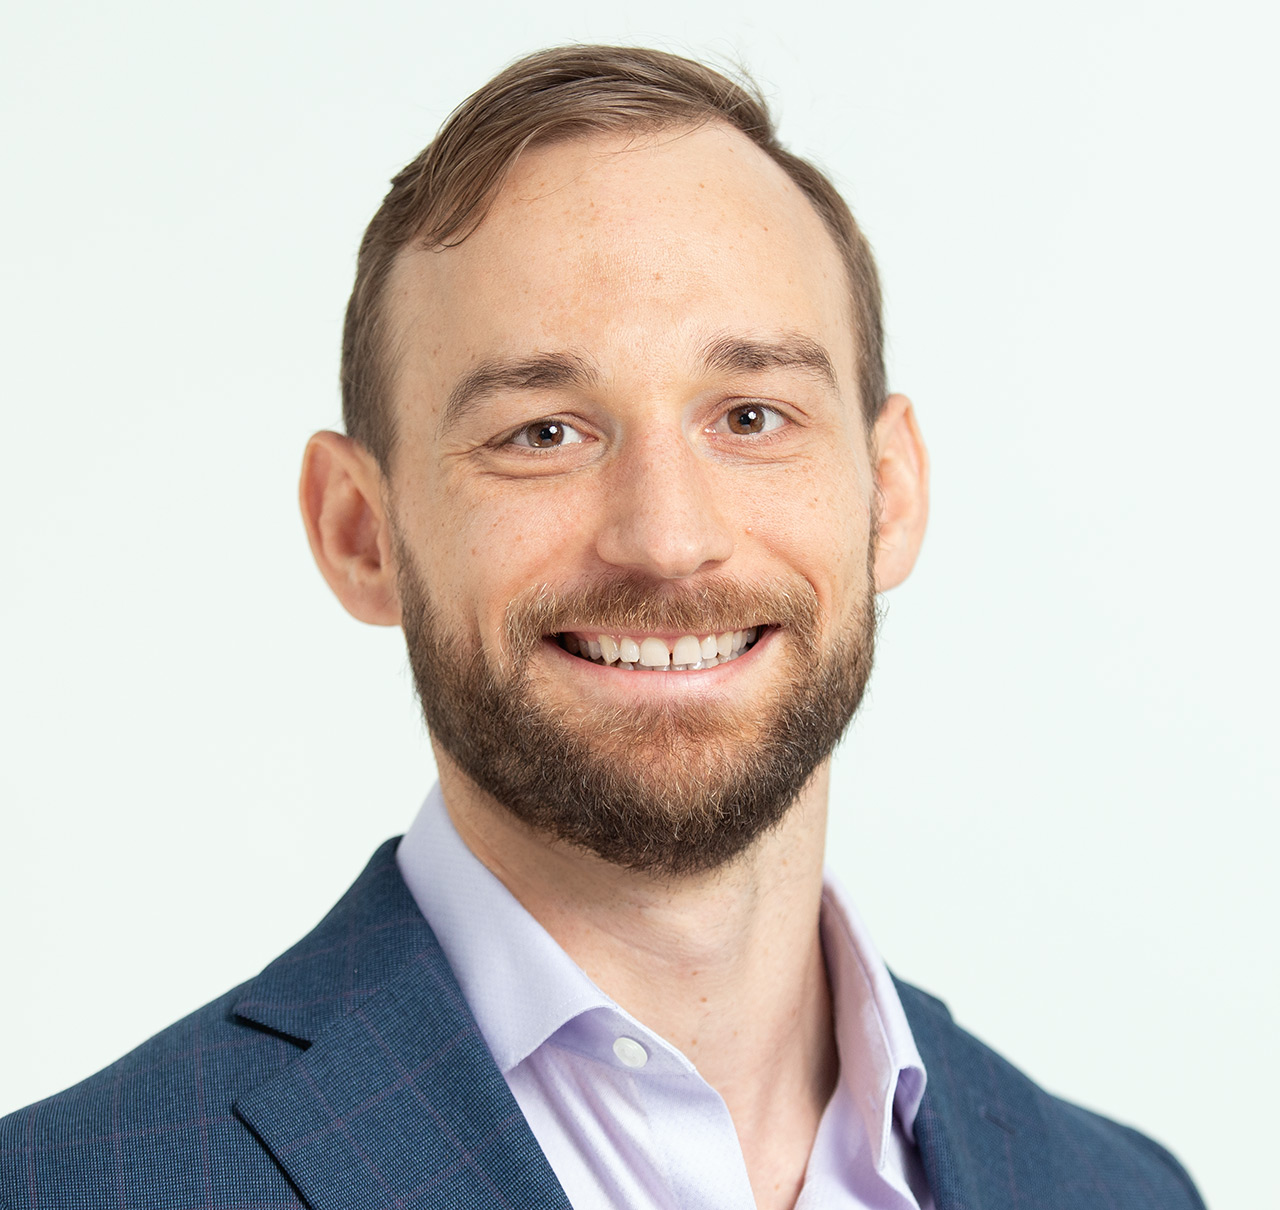
\includegraphics[width=0.28\linewidth,height=\textheight,keepaspectratio,alt={Karan}]{./images/about/karan.png}

}

\caption{Karan}

\end{figure}%

Karan is a member of the OR 568 Machine Learning Project team. Add a
short professional biography here describing academic background,
current role, technical interests, and contributions to the project. You
can also include research interests, relevant industry experience, and
what Karan is focusing on within the team.

\section{\texorpdfstring{\href{https://your-link-here.com}{Irena
Austin}}{Irena Austin}}\label{irena-austin}

\begin{figure}[H]

{\centering 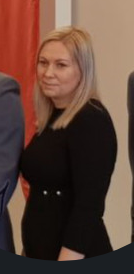
\includegraphics[width=0.28\linewidth,height=\textheight,keepaspectratio,alt={Irena}]{./images/about/irena.png}

}

\caption{Irena}

\end{figure}%

I am a Human Resources professional in the federal sector currently
pursuing a master's in Management and Responsible AI at George Mason
University. My work focuses on bridging the gap between traditional HR
operations and predictive analytics. In this repository, I apply machine
learning models to analyze complex datasets like flight delays and
organizational risk.

\section{\texorpdfstring{\href{https://your-link-here.com}{Val
Lastname}}{Val Lastname}}\label{val-lastname}

\begin{figure}[H]

{\centering 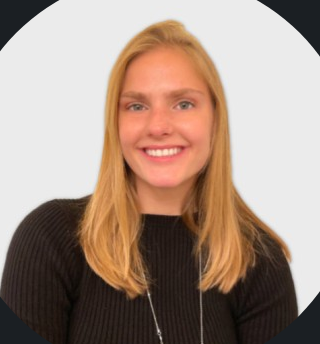
\includegraphics[width=0.28\linewidth,height=\textheight,keepaspectratio,alt={Val}]{./images/about/val.png}

}

\caption{Val}

\end{figure}%

Val is a member of the OR 568 Machine Learning Project team. Add a short
biography here describing technical background, work experience,
academic interests, and role on the project team. This can include
domain interests, tools, modeling focus, or collaboration strengths.




\end{document}
